\documentclass{beamer}

\setbeamertemplate{frametitle}[default][center]

\usepackage{graphicx}
\usepackage{hyperref}


%\usepackage{verbatim}

\definecolor{mymagenta}{rgb}{0.9, 0, 0.9}

\newcommand{\msmagenta}[1]{{\color{mymagenta} #1}}


\begin{document}

\title{``Request for Plot":\\ is {\bf softmax cross-normalization}\\ fruitful in transformers?}
\author{Mishka (Michael Bukatin)}

\date
{\footnotesize 
Dataflow Matrix Machines project\\[2ex]

\href{https://github.com/anhinga}{\tt https://github.com/anhinga}\\[2ex]

\msmagenta{I am looking for collaborators}
}

\begin{frame}
  \titlepage
\end{frame}

\begin{frame}

\frametitle{``Request for Plot"}

Replace\\[2ex]

\hspace{0.5in}Attention($Q, K, V$) = softmax($cKQ^\text{T}$)$V$\\[2ex]

with\\[2ex]

\hspace{0.5in}Attention($Q, K, V$) = softmax($cKQ^\text{T}$)\msmagenta{softmax$^\text{T}$}($V$)\\[4ex]

Does your favorite learning curve improve?\\[8ex]

Why do I think this is a good shot?


\end{frame}

\begin{frame}

\frametitle{Why this might be a good idea?}

I experimented with interpreting monochrome images as matrices
and multiplying those matrices via matrix product and
checking whether results are visually interesting.\\[2ex]

{\bf Multiplying monochrome images as matrices:\\ A*B and softmax}\\[2ex]

\href{https://github.com/anhinga/JuliaCon2021-poster}{\tt https://github.com/anhinga/JuliaCon2021-poster}\\[2ex]


\end{frame}


\begin{frame}

\includegraphics[scale=0.18]{p12}

In Transformers people sometimes {\bf softmax} rows of the left matrix:
{\scriptsize Attention($Q, K, V$) = softmax($cKQ^T$)$V$ from ``Attention Is All You Need" (2017).}\\[1ex]

In the second example we {\bf softmax} rows of the left matrix {\bf and} \msmagenta{columns of the right matrix} resulting in products
with richer,\\ more fine-grained structure.

\end{frame}

\begin{frame}

\includegraphics[scale=0.18]{p34}

In Transformers people sometimes {\bf softmax} rows of the left matrix:
{\scriptsize Attention($Q, K, V$) = softmax($cKQ^T$)$V$ from ``Attention Is All You Need" (2017).}\\[1ex]

In the second example we {\bf softmax} rows of the left matrix {\bf and} \msmagenta{columns of the right matrix} resulting in products
with richer,\\ more fine-grained structure.

\end{frame}

\begin{frame}


\includegraphics[scale=0.5]{symmetric}

\end{frame}

\begin{frame}

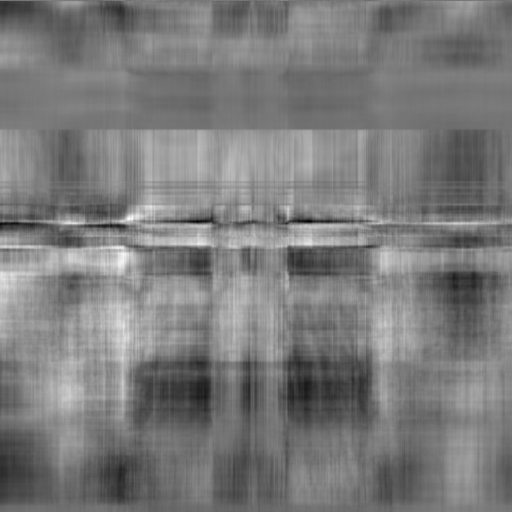
\includegraphics[scale=0.5]{asymmetric}

\end{frame}

\begin{frame}

\frametitle{Cross-normalization}

{\LARGE softmax\msmagenta{$^\text{T}$}($V$)}\\[2ex]

\includegraphics[scale=0.5]{cross-norm}\\[2ex]

values are horizontal stripes\\[2ex]

{\bf cross-norm:} softmax vertical vectors\\[2ex]

a vertical vector consists of $i$'s coords of all values for a given $i$



\end{frame}

\begin{frame}

\frametitle{Contact}

Open an issue in\\[2ex]

\href{https://github.com/anhinga/JuliaCon2021-poster}{\tt https://github.com/anhinga/JuliaCon2021-poster}\\[2ex]


or send an e-mail to bukatin @ cs dot brandeis dot edu



\end{frame}




\end{document}